\documentclass[smallextended]{svjour3}
%\usepackage{cite}
% *** GRAPHICS RELATED PACKAGES ***
%
  \usepackage[pdftex]{graphicx}
%
\usepackage[cmex10]{amsmath}

% *** ALIGNMENT PACKAGES ***
%
\usepackage{array}
%\usepackage{fixltx2e}

\usepackage{stfloats}
% LaTeX2e). It also provides a command:
\fnbelowfloat
\usepackage{endfloat}
\usepackage{booktabs}
\usepackage{amssymb}
\usepackage{amsmath}
\usepackage{pgf}
\usepackage{tikz}
\usetikzlibrary{arrows,positioning}
\usepackage[hyphens]{url}
\usepackage{color}
\usepackage{graphicx}
\usepackage{xspace}
\newcommand*{\eg}{e.g.\@\xspace}
\newcommand*{\ie}{i.e.\@\xspace}
\newcommand*{\vs}{vs.\@\xspace}

\newcommand*{\EMD}{\mathrm{EMD}}

% correct bad hyphenation here
\hyphenation{wave-let}

\usepackage{color}
\newcommand{\vl}[1]{\textcolor{orange}{Vincent : #1}}
\newcommand{\gl}[1]{\textcolor{red}{Gr\'egoire : #1}}
\newcommand{\ja}[1]{\textcolor{magenta}{Joakim : #1}}
\newcommand{\ml}[1]{\textcolor{blue}{ Mathieu : #1}}

\usepackage[backend=bibtex,style=numeric-comp,sorting=none,firstinits=true]{biblatex}
\bibliography{biblio}
%\renewcommand{\baselinestretch}{2}


\begin{document}
%
% paper title
% can use linebreaks \\ within to get better formatting as desired
% Do not put math or special symbols in the title.
%\title{An evaluation framework for event detection using a morphological model of acoustic scenes}
\title{Relevance-based Quantization of Scattering Features for Unsupervised Mining of Environmental Audio}
\titlerunning{Relevance-based Quantization of Scattering Features}


\author{Vincent Lostanlen         \and
		Gr\'egoire Lafay  \and Joakim And\'en  \and Mathieu Lagrange.}

\institute{Vincent Lostanlen \at
              \email{vincent.lostanlen@nyu.edu}
\and
			Gr\'egoire Lafay \at
              \email{lafaygregoire@gmail.com}
\and
			Joakim And\'en \at
              \email{janden@flatironinstitute.org}           \and
			Mathieu Lagrange \at
              \email{mathieu.lagrange@cnrs.fr}
}

\date{Received: date / Accepted: date}
% The correct dates will be entered by the editor



% make the title area
\maketitle

% As a general rule, do not put math, special symbols or citations
% in the abstract or keywords.
\begin{abstract}
The emerging field of computational acoustic monitoring aims at retrieving high-level information from acoustic scenes recorded by some network of sensors. These networks gather large amounts of data requiring analysis. To decide which parts to inspect further, we need tools that automatically mine the data, identifying recurring patterns and isolated events. This requires a similarity measure for acoustic scenes that does not impose strong assumptions on the data.

The state of the art in audio similarity measurement is the ``bag-of-frames'' approach, which models a recording using summary statistics of short-term audio descriptors, such as mel-frequency cepstral coefficients (MFCCs). They successfully characterise static scenes with little variability in auditory content, but cannot accurately capture scenes with a few salient events superimposed over static background.
To overcome this issue, we propose a two-scale representation which describes a recording using clusters of scattering coefficients. The scattering coefficients capture short-scale structure, while the cluster model captures longer time scales, allowing for more accurate characterization of sparse events. Evaluation within the acoustic scene similarity framework demonstrates the interest of the proposed approach.
\keywords{
unsupervised learning \and data mining \and acoustic signal processing \and wavelet transforms \and audio databases \and content-based retrieval \and nearest neighbor searches \and acoustic sensors \and environmental sensors.}
% \PACS{PACS code1 \and PACS code2 \and more}
\end{abstract}


\section{Introduction}

The amount of audio data recorded from our sonic environment has grown considerably over the past decades.
In order to measure the effect of human activity and climate change on animal biodiversity~\cite{sueur2015ecoacoustics}, researchers have recently undertaken a massive deployment of acoustic sensors throughout the world~\cite{warren2006urban, NessSST13, stowell13b}.
In addition, recent work has explored acoustic monitoring for characterization of human pleasantness in urban areas~\cite{guyot2005urban, ricciardi2015sound}, as well as the prediction of annoyance due to traffic~\cite{gloaguen}.
Since they bear a strong societal impact and raise many scientific challenges, we believe that these applications are of considerable interest for signal processing community.

%These questions are explored in an emerging field of computational bioacoustics, known as ecoacoustics, which is the interdisciplinary study of relationships between natural or anthropogenic sounds and their environments at the intersection of ecology, acoustics and computer science . %~\cite{wimmer2013sampling}

An important problem is that manually analysing the recorded data to identify the quantities of interest is very costly. Some sort of pre-screening is therefore required to reduce the need for human expert listening and annotation.
To this aim, the most straightforward approach is to specify a closed set of sound classes, such as sounds classes expected to appear near the acoustic sensors. Computational models are then trained  for these classes which are used to automatically annotate recordings~\cite{quteprints96243}. A given time interval (\eg{} a single day) is then represented by the number of events detected during that interval for each class. This allows the scientist to drastically reduce the amount of information requiring manual processing. However, this approach has two drawbacks. First, it relies on trained models whose prediction on unseen data -- \ie{} sensors outside of the training set -- is prone to errors. Secondly, and more importantly, it is based on prior knowledge and thus cannot be considered for exploratory analysis, in which quantities of interest have yet to be defined.

To identify which parts need human inspection, one needs tools that are able to detect both recurring patterns and sparsely distributed events. Identifying recurring patterns allows the user to focus on certain time points for manual annotation, while detection of more rare structures enables discovery of unforeseen phenomena.

With this aim, we need to design an algorithm for acoustic similarity retrieval, where the audio fragments judged ``most similar'' to a given query recording must be extracted from some larger dataset. To construct such an algorithm, we are required to represent an audio recording in a way that captures its distinctive qualities. A widespread choice of representation is the bag of frames~\cite{aucouturier2007bag}, which describes an auditory scene recording using summary statistics of short-time features. Unfortunately, the bag-of-frames approach only captures the average structure of the scene, so the approach often fails when presented with highly dynamic scenes or those characterised by a few distinct sound events sparsely distributed over time. Furthermore, experiments in cognitive psychology~\cite{dubois2006cognitive} and cognitive neuroscience~\cite{nelken2004processing} suggest that human acoustic perception is highly sensitive to such isolated sound events. We believe that the failure to model such distinct events is one of the reasons why the bag-of-frames representation is insufficient~\cite{lagrange:hal-01082501}.

Solving the acoustic similarity retrieval first requires the ability to capture meaningful signal structure at small time scales.
This is often achieved using mel-frequency cepstral coefficients (MFCCs).
Originally developed for speech processing~\cite{davis-mermelstein}, MFCCs have recently found wider use in music information retrieval~\cite{logan} and environmental audio processing~\cite{aucouturier2007bag}.
A richer representation, the scattering transform, has enjoyed significant success in various audio~\cite{Anden2014} and biomedical~\cite{chudacek} signal classification tasks.
Its structure is that of a convolutional neural network~\cite{lee,lostanlen-deep-spiral,soundnet,arandjelovic-zisserman}, but with fixed filters.
Specifically, it alternates convolutions with wavelet filters and pointwise nonlinearities to ensure time-shift invariance and time-warping stability~\cite{Mallat2012}.

For our task, one advantage of the scattering transform is that it does not require a training step, allowing for a wider range of applications compared to learned features. Indeed, for data mining of previously unheard datasets, the properties of relevant audio structures remains to be defined, leading to an unsupervised setting.

In this work, we propose a new model for acoustic scenes, where the signal is represented at sub-second scales by scattering transforms, while larger scales are captured by a cluster model. This unsupervised model quantizes the scattering coefficients into a given number of clusters. These clusters are then used to define a set of distances for acoustic similarity retrieval. Evaluating this approach on a scene retrieval task, we obtain significant improvements over traditional bag-of-frames and summary statistics models applied both to MFCCs and scattering coefficients.

Motivations of the proposed approach and a brief review of the state of the art in acoustic scene modeling are given in Section~\ref{sec:soa}. We describe the scattering transform in Section~\ref{sec:scattering}, discuss feature post-processing in Section~\ref{sec:design} and propose a cluster-based scene description in Section~\ref{sec:object}. Section~\ref{sec:experiments} describes several experiments for the acoustic scene similarity retrieval task. Results are reported in Section~\ref{sec:results}.

\section{Background} \label{sec:soa}

%Computational bioacoustics refers to the numerical investigation of sound production, dispersion and reception in animals, including humans. A recent paradigm processes the audio stream in a holistic way over large time scales, without assuming that a single species is present throughout the recording. Automated systems within this paradigm attempt to infer global properties of bioacoustic scenes, including biodiversity indices~\cite{Bardeli2010} and migration patterns~\cite{Obrist2010}. They also mark time intervals of particular interest for detailed human inspection~\cite{rosenstock2002landbird}.

Caracterization of the similarity between audio recordings be they at the scale of the minute, the hour, the day or larger is of interest for many applications areas involving acoustic monitoring such as urban sound environment analysis and ecoacoustics. In this context, a classical approach is the bag of frames (BoF), first applied to the problem by Aucouturier et al.~\cite{aucouturier2007bag}.
It models an auditory scene using high-level summary statistics computed from local features, typically implemented by Gaussian mixture models (GMMs) of MFCCs.

It is worth mentionning that this task typically falls into a unsupervised paradigm where no prior knowldge is used to model a given scene. For each scene $s$, a model is compute $M_s$ is computed. The similarity among the scene $s_1$ and $s_2$ is computed as the similarity, see Section~\ref{sec:experiments} for further details. The BoF approach is also widely used in a supervised fashion for solving a classification task~\cite{7100934}. In this case, each class of scenes from a given typology, say \{\emph{park, boulevard, square}\}, is modeled by a GMM trained on scenes taken from a training set. In order to predict the class of a given scene $s$, the likelihood each model given the scene are computed. The scene is then labeled park if the likelihood of the GMM trained on park scenes is higher than all other likelihoods.

While BoF has largely been superseded by more sophisticated methods for the task of acoustic scene classification~\cite{7100934}, it remains the best-performing model for acoustic scene similarity retrieval.
Though, this representation was recently shown to perform comparably to direct averaging of the features for a variety of datasets~\cite{lagrange:hal-01082501}.
This contrasts with the typical morphology of acoustic scenes, a ``skeleton of events on a bed of textures,'' where a few discrete sound events are superimposed upon a stationary acoustic background~\cite{nelken2013}.
Such events are not well-characterised by summarizing short-term features, but are better described by large-scale temporal evolution of auditory scenes.
The latter approach should therefore prove more fruitful in measuring auditory scene similarity.

This statement has some support in auditory psychology as well as sound synthesis based on summary statistics~\cite{mcdermott2013summary}. Studies in the cognitive psychology of urban sound environments have shown that global sound level (perceived or measured) is not sufficient to fully characterise an acoustic scene~\cite{guyot2005urban,kang2006urban}. Instead, cognitive processes such as sound environment quality perception~\cite{dubois2006cognitive} or loudness judgment~\cite{kuwano_memory_2003} seem to rely upon higher-level cognitive attributes. These typically include the identities of the sound sources which constitute the scene. It has been shown that, if available, the complete description of the scene in terms of event occurrences is powerful enough to reliably predict high-level cognitive classes. For example, in urban areas the presence of birds is likely to be heard in parks and are therefore strong pleasantness indicators. Consequently, research in sound perception is now strongly focused on the contribution of specific sound sources in the assessment of sound environments~\cite{ricciardi2015sound,lavandier2006contribution}. Although the complete set of events occurring within a given auditory stream may not be discernable even to human expects, research has shown that a small set of events (so-called markers) suffice to reliably predict many high-level attributes.

From a cognitive psychology perspective, the consensus is therefore that only a few distinct events are sufficient to describe an auditory scene, in contrast to BoF models which treat each observation separately and do not capture their temporal structure. A method that takes this knowledge into account could therefore have potential for great impact in acoustic scene modeling, given a rich enough representation of these distinct events.

\section{Wavelet scattering \label{sec:scattering}}

Local invariance to time-shifting and stability to time-warping are necessary when representing acoustic scenes for similarity measurement.
The scattering transform is designed to satisfy these properties while retaining high discriminative power.
It is computed by applying auditory and modulation wavelet filter banks alternated with complex modulus nonlinearities.

\subsection{Invariance and stability in audio signals}
The notion of invariance to time-shifting plays an essential role in acoustic scene similarity retrieval.
Indeed, recordings may be shifted locally in time without affecting similarity to other recordings.
To discard this superfluous source of variability, signals are first mapped into a time-shift invariant feature space. These features are then used to calculate similarities. Since the features ensure invariance, it does not have to be learned when constructing the desired similarity measure.

Formally, given a signal $\boldsymbol{x}(t)$, we would like its translation $\boldsymbol{x_c}(t) = \boldsymbol{x}(t-c)$ to be mapped to the same feature vector provided that $|c| \ll T$ for some maximum duration $T$ that specifies the extent of the time-shifting invariance. We can also define more complicated transformations by letting $c$ vary with $t$. In this case, we have $\boldsymbol{x_\tau}(t) = \boldsymbol{x}(t-\tau(t))$ for some function $\tau$, which performs a time-warping of $\boldsymbol{x}(t)$ to obtain $\boldsymbol{x_\tau}(t)$. Time-warpings model various changes, such as small variations in pitch, reverberation, and rhythmic organization of events. These make up an important part of intra-class variability among natural sounds, so representations must be robust with respect to such transformations.

The wavelet scattering transform, described below, has both of these desired properties: invariance to time-shifting and stability to time-warping. The stability condition can be formulated as a Lipschitz continuity property, which guarantees that the feature transforms of $\boldsymbol{x}(t)$ and $\boldsymbol{x_\tau}(t)$ are close together if $|\tau'(t)|$ is bounded by a small constant \cite{Mallat2012}.

\subsection{Wavelet scalogram}
Our convention for the Fourier transform of a continuous-time signal $\boldsymbol{x}(t)$ is $\boldsymbol{\hat{x}}(\omega) = \int_{-\infty}^{+\infty} x(t) \exp(- \mathrm{i} 2\pi \omega t) \, \mathrm{d}t$.
Let $\boldsymbol{\psi}(t)$ a complex-valued analytic bandpass filter of
central frequency $\xi_1$ and bandwidth $\xi_1/Q_1$, where $Q_1$ is the quality factor of the filter.
A filter bank of wavelets is built by dilating $\boldsymbol{\psi}(t)$
according to a geometric sequence of scales $2^{\gamma_1/Q_1}$, obtaining
\begin{equation}
\boldsymbol{\psi_{\gamma_1}}(t) = 2^{-\gamma_1/Q_1} \boldsymbol{\psi}(2^{-\gamma_1/Q_1} t)\mbox{.}
\end{equation}
The variable $\gamma_1$ is a scale (an inverse log-frequency) taking integer values between $0$ and $(J_1 Q_1 - 1)$, where $J_1$ is the number of octaves spanned by the filter bank.
For each $\gamma_1$, the wavelet $\boldsymbol{\psi_{\gamma_1}}(t)$
has a central frequency of $2^{-\gamma_1/Q_1}\xi_1$ and a bandwidth of $2^{-\gamma_1/Q_1}\xi_1/Q_1$ resulting in the same quality factor $Q_1$ as $\boldsymbol{\psi}$.
In the following, we set $\xi_1$ to $20~\mathrm{kHz}$, $J_1$ to $10$, and the quality factor $Q_1$, which is also the number of wavelets per octave, to $8$. This results in the wavelet filters covering the whole range of human hearing, from $20~\mathrm{Hz}$ to $20~\mathrm{kHz}$. Setting $Q_1 = 8$ results in filters whose bandwidth approximates an equivalent rectangular bandwidth (ERB) scale~\cite{Fastl2007}.

The wavelet transform of an audio signal
$\boldsymbol{x}(t)$ is obtained by convolution with all wavelet filters.
Applying a pointwise complex modulus the transform yields
the wavelet scalogram
\begin{equation}
\boldsymbol{x_1}(t, \gamma_1)
= \vert \boldsymbol{x} \ast \boldsymbol{\psi_{\gamma_1}} \vert (t)\mbox{.}
\end{equation}
The scalogram bears resemblance to the constant-Q transform (CQT),
which is derived from the short-term Fourier transform (STFT) by averaging the frequency
axis into constant-Q subbands of central frequencies $2^{-\gamma_1/Q_1}\xi_1$.
Indeed, both time-frequency representations are indexed by time $t$ and log-frequency $\gamma_1$.
However, contrary to the CQT, the scalogram reaches a better time-frequency localization across the whole
frequency range, whereas the temporal resolution of the traditional CQT is fixed by the support of the STFT analyzing window. %\cite{Brown1992}
Therefore, the scalogram has a better temporal localization at high
frequencies than the CQT, at the expense of a greater computational cost
since the inverse fast Fourier transform routine must be called for each wavelet $\boldsymbol{\psi_{\gamma_1}}$ in the filter bank.
However, this allows us to observe amplitude modulations at fine temporal scales in the scalogram, down to $2Q_1/\xi_1$ for $\gamma_1 = 0$, of the order of $1\,\textrm{ms}$ given the aforementioned values of $Q_1$ and $\xi_1$.

To obtain the desired invariance and stability properties, the scalogram is averaged in time using a lowpass filter $\boldsymbol{\phi}(t)$ with cut-off frequency $1/T$ (and approximate duration $T$), to get
\begin{equation}
\mathbf{S_1}\boldsymbol{x}(t, \gamma_1) = \boldsymbol{x_1}(\cdot, \gamma_1) \ast \boldsymbol{\phi}(t),
\end{equation}
which is known as the set of first-order scattering coefficients. They capture the average spectral envelope of $\boldsymbol{x}(t)$ over scales of duration $T$ and where the spectral resolution varying with constant Q. In this way, they are closely related to the mel-frequency spectrogram and related features, such as MFCCs.

\subsection{Extracting modulations with second-order scattering}
In auditory scenes, short-time amplitude modulations may be caused by a variety of rapid mechanical interactions, including collision, friction, turbulent flow, and so on.
At longer time-scales, they also account for higher-level attributes of sound, such as prosody in speech or rhythm in music.
Although they are discarded while filtering $\boldsymbol{x_1}(t,\gamma_1)$ into the time-shift invariant representation $\mathbf{S_1}\boldsymbol{x}(t,\gamma_1)$, they can be recovered from $\boldsymbol{x_1}(t,\gamma_1)$ by a second wavelet transform and another complex modulus.

We define second-order wavelets $\boldsymbol{\psi_{\gamma_2}}(t)$ in the same way as the first-order wavelets, but with parameters $\xi_2$, $J_2$, and $Q_2$. Consequently, they have central frequencies $2^{-\gamma_2/Q_2}\xi_2$ for $\gamma_2$ taking values between $0$ and $(J_2 Q_2 - 1)$. While this abuses notation slightly, the identity of the wavelets should be clear from context.
The amplitude modulation spectrum resulting from a wavelet modulus decomposition using these second-order wavelets is then
\begin{equation}
\boldsymbol{x_2}(t,\gamma_1,\gamma_2) =
\vert \boldsymbol{x_1} \ast \boldsymbol{\psi_{\gamma_2}} \vert(t,\gamma_1).
\end{equation}
In the following, we set $\xi_2$ to $2.5\,\mathrm{kHz}$, $Q_2$ to $1$, and $J_2$ to $12$. Lastly, the low-pass filter $\boldsymbol{\phi}(t)$ is applied to $\boldsymbol{x_2}(t, \gamma_1, \gamma_2)$ to guarantee local invariance to time-shifting, which yields the second-order scattering coefficients
\begin{equation}
\mathbf{S_2}\boldsymbol{x}(t,\gamma_1,\gamma_2) =
\boldsymbol{x_2}(\cdot,\gamma_1,\gamma_2) \ast \boldsymbol{\phi}(t).
\end{equation}

The scattering transform $\mathbf{S}\boldsymbol{x}(t,\gamma)$ consists of the concatenation of first-order coefficients $\mathbf{S_1}\boldsymbol{x}(t,\gamma_1)$ and second-order coefficients $\mathbf{S_2}\boldsymbol{x}(t,\gamma_1,\gamma_2)$ into a feature matrix $\mathbf{S}\boldsymbol{x}(t,\gamma)$, where $\gamma$ denotes either $\gamma_1$ or $(\gamma_1,\gamma_2)$. While higher-order scattering coefficients can be calculated, for the purposes of our current work, the first and second order are sufficient.
Indeed, higher-order scattering coefficients have been shown to contain reduced energy and are therefore of limited use~\cite{irene}.

\subsection{Gammatone wavelets}
\begin{figure}
\begin{center}
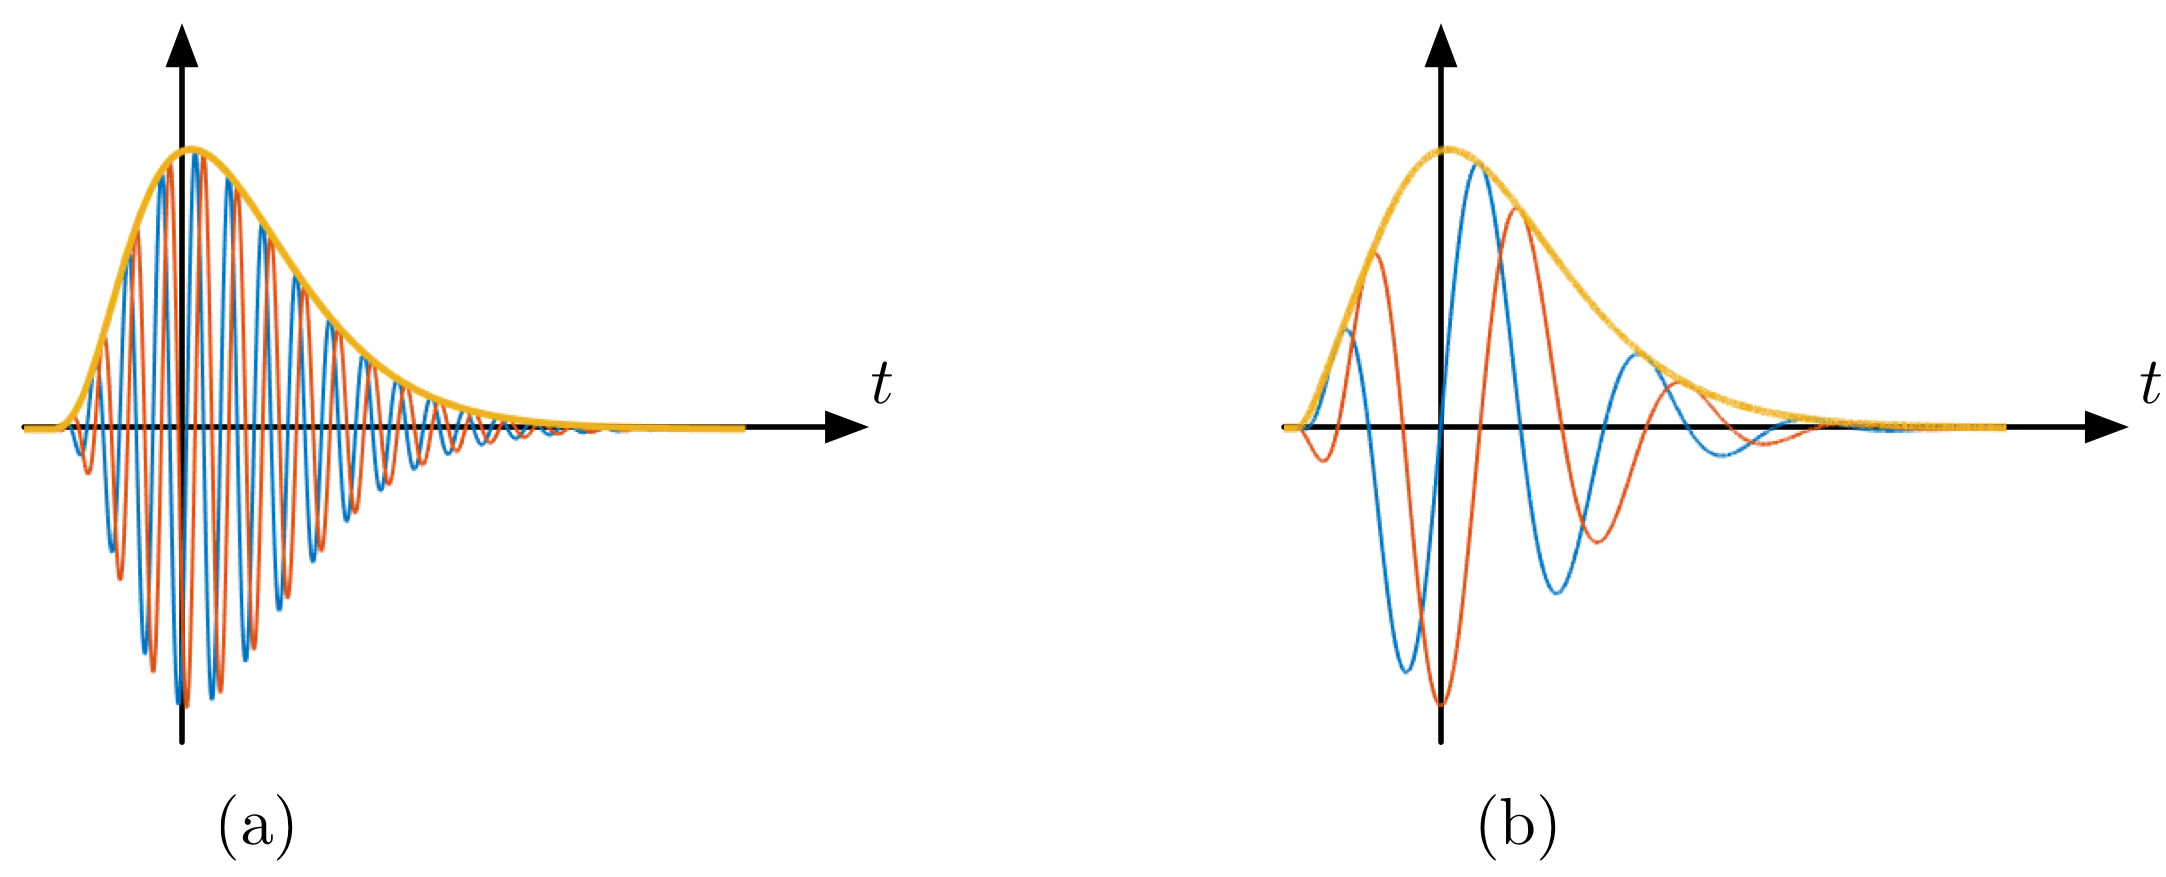
\includegraphics[width=\columnwidth]{figures/gammatones}
\caption{
\label{fig:gammatones}
Gammatone wavelets $\boldsymbol{\psi}(t)$ in the time domain with quality factors (a) $Q = 4$ and (b) $Q = 1$.
Oscillations (red, blue) are the real and imaginary parts. The envelope (yellow) is the complex modulus.}
\end{center}
\end{figure}
Wavelets
$\boldsymbol{\psi_{\gamma_1}}(t)$ and $\boldsymbol{\psi_{\gamma_2}}(t)$ are designed as fourth-order Gammatone
wavelets with one vanishing moment~\cite{Venkitaraman2014}, and are shown in Figure~\ref{fig:gammatones}.
In the context of auditory scene analysis, the asymmetric envelopes of Gammatone wavelets are more biologically plausible than the symmetric, Gaussian envelopes of the more widely used Morlet wavelets.
Indeed, it allows to reproduce two important psychoacoustic effects in the mammalian cochlea: the asymmetry of temporal masking and the asymmetry of spectral masking~\cite{Fastl2007}.
The asymmetry of temporal masking is the fact that a masking noise has to be louder if placed after the onset of a stimulus rather than before.
Likewise, because critical bands are skewed towards higher frequencies, a masking tone has to be louder if it is above the stimulus in frequency rather than below.
It should also be noted that Gammatone wavelets follow the typical amplitude profile of natural sounds, beginning with a relatively sharp attack and ending with a slower decay.
As such, they are similar to filters discovered automatically by unsupervised encoding of natural sounds~\cite{Smith2006,sainath2015interspeech}.
In addition, Gammatone wavelets have proven to outperform Morlet wavelets on a benchmark of supervised musical instrument classification from scattering coefficients \cite{lostanlen2017phd}.
This suggests that, despite being hand-crafted and not learned, Gammatone wavelets provide a sparser time-frequency representation of acoustic scenes compared to other variants.

\section{Feature design}
\label{sec:design}

Before constructing models for similarity estimation, it is beneficial to process scattering coefficients to improve invariance, normality, and generalization power.
In this section, we review two transformations which achieve these properties: logarithmic compression and standardisation.

\subsection{Logarithmic compression}
\label{sec:logcomp}

Many algorithms in pattern recognition, including nearest neighbor classifiers and support vector machines, tend to work best when all features follow a standard normal distribution across all training instances~\cite{Hsu2003}.
Yet the distribution of the scattering coefficients is skewed towards larger values. We can reduce this skewness by applying a pointwise concave transformation to all coefficients. In particular, we find that the logarithm performs particularly well in this respect.
Figure~\ref{fig:histograms} shows the distribution of an arbitrarily chosen scattering coefficient over the DCASE 2013 dataset, before and after logarithmic compression.

\begin{figure}
\begin{center}
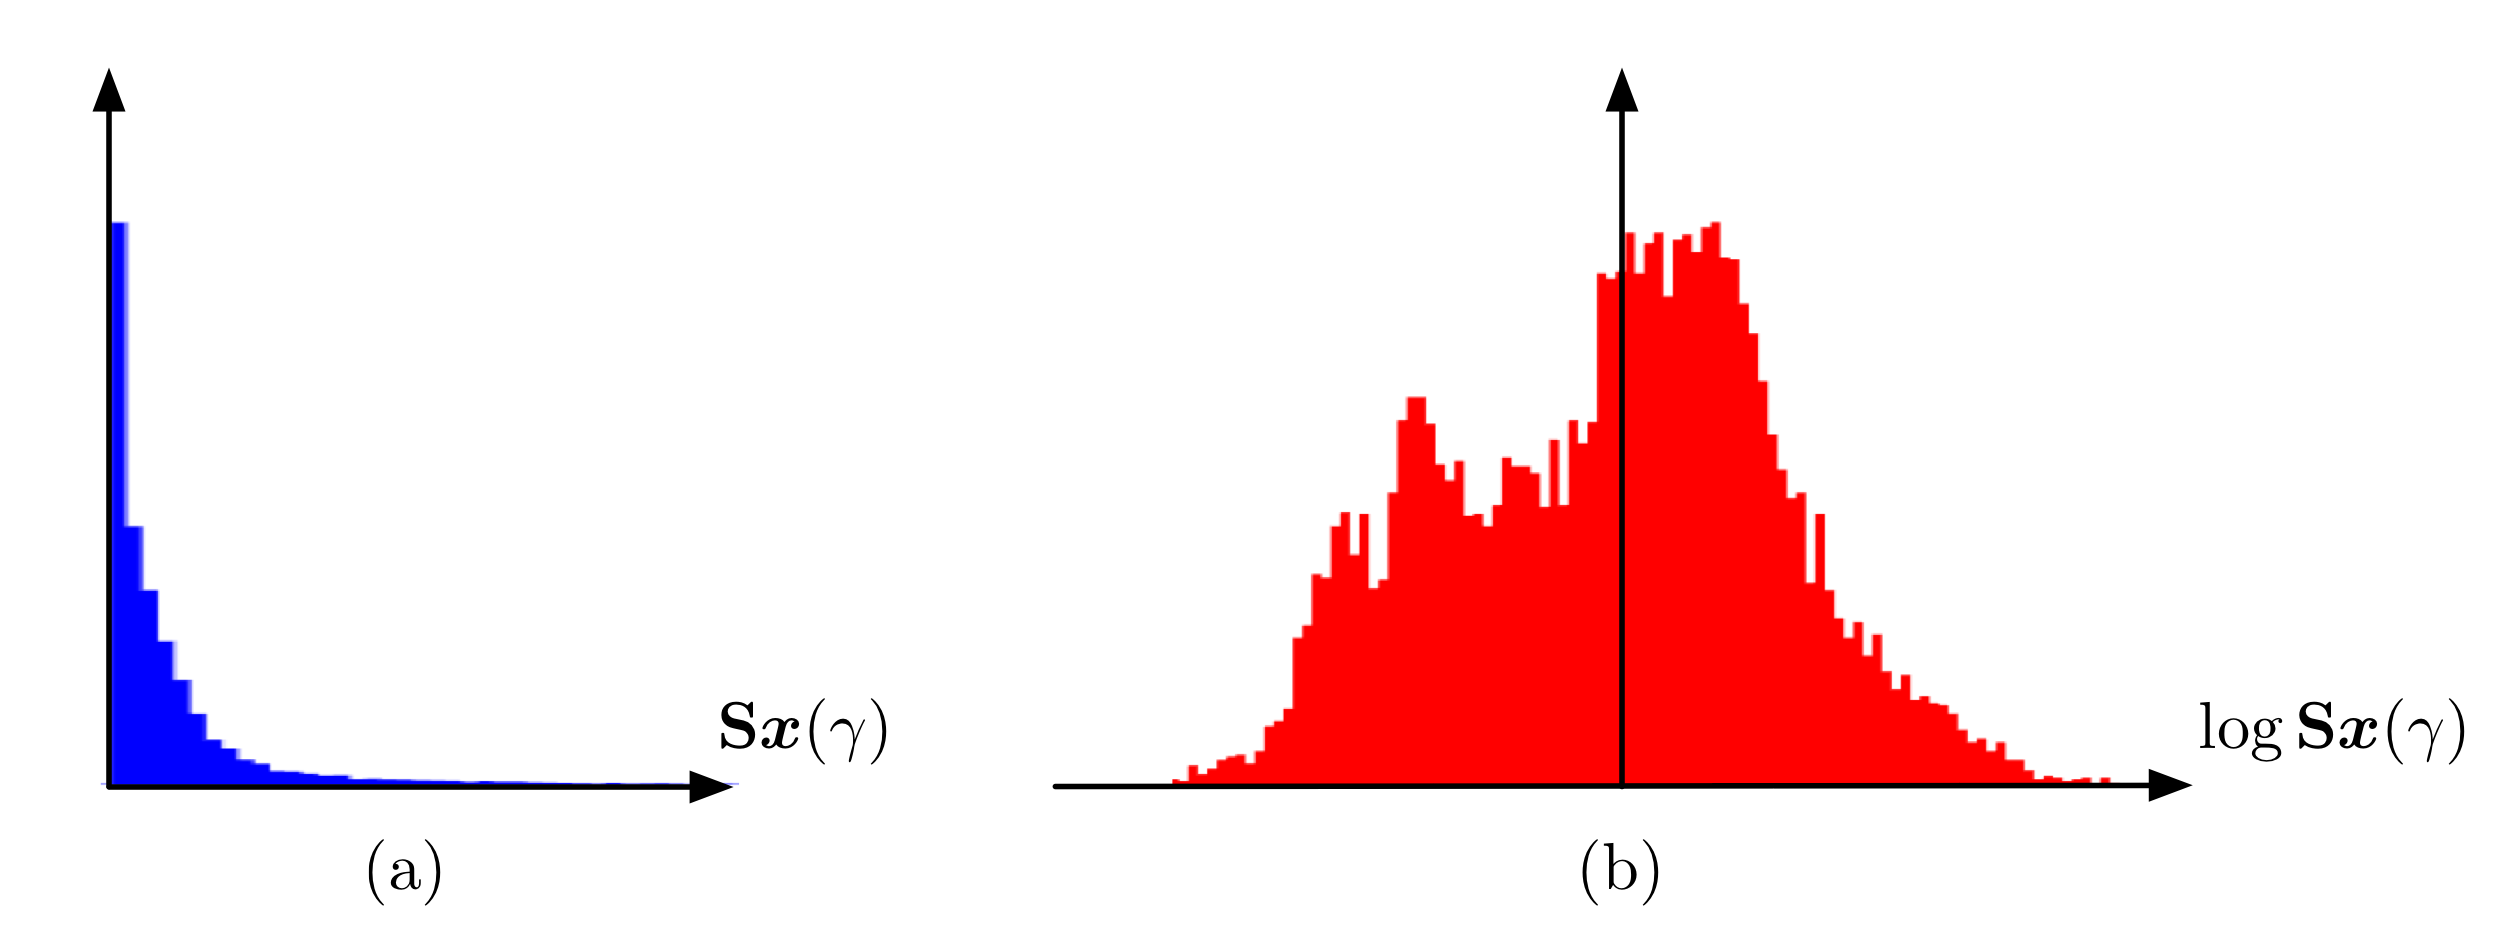
\includegraphics[width=\columnwidth]{figures/compression}
\caption{
\label{fig:histograms}
Histogram of values taken by the first-order scattering coefficient $\mathbf{S}\boldsymbol{x}(\gamma)$, corresponding to a central acoustic frequency of $302\,\mathrm{Hz}$,
(a) before and (b) after logarithmic compression.}
\label{fig:compression}
\end{center}
\end{figure}

Taking the logarithm of a magnitude spectrum is ubiquitous in audio signal processing.
Indeed, it is corroborated by the Weber-Fechner law in psychoacoustics, which states that the sensation of loudness is roughly proportional to the logarithm of the acoustic pressure.
We must also recall that the measured amplitude of sound sources often decays polynomially with the distance to the microphone--a source of spurious variability in scene classification.
Logarithmic compression linearise this dependency, facilitating the construction of powerful invariants at the classifier stage.

\subsection{Standardisation}
\label{sec:stand}

Let $\mathbf{S}\boldsymbol{x}(\gamma,n)$ be a dataset, where $\gamma$ and $n$ denote feature and sample indices, respectively.
Many algorithms operate better on features which have zero mean and unit variance to avoid mismatch in numeric ranges~\cite{Hsu2003}.
To standardise $\mathbf{S}\boldsymbol{x}(\gamma,n)$, we subtract the sample mean vector $\mu[\mathbf{S}\boldsymbol{x}(\gamma)]$ from $\mathbf{S}\boldsymbol{x}(\gamma,n)$ and divide the result by the sample standard deviation vector $\sigma[\mathbf{S}\boldsymbol{x}] (\gamma)$.
The vectors $\mu[\mathbf{S}\boldsymbol{x}(\gamma)]$ and $\sigma[\mathbf{S}\boldsymbol{x}](\gamma)$ are estimated from the entire dataset.

\section{Acoustic scene similarity retrieval}
\label{sec:object}

%As part of the aforementioned research areas and applications, the emerging field of \emph{Acoustic Scene Analysis} (also called \emph{Sound Scene Analysis})~\cite{Stowell15} aims to develop approaches and systems for the automatic analysis of environmental sounds and soundscapes (originating both from urban or nature environments). While research methodologies in related fields such as Automatic Speech Recognition (ASR)~\cite{Rabiner93} and Music Information Retrieval (MIR)~\cite{Muller07} are now well established, research addressing Acoustic Scene Analysis remains relatively young.

%From a data processing point of view, a holistic scheme, such as the bag-of-frame approach~\cite{aucouturier2007bag}, has a simplicity, but clearly face poor performance on realistic conditions~\cite{lagrange:hal-01082501}.

As discussed in Section~\ref{sec:soa}, results in sound perception suggest the appropriateness of source-driven representations of auditory scenes for predicting high-level properties. While this can be addressed in the supervised case using late integration of discriminative classifiers~\cite{Anden2014}, this is not directly feasible in the unsupervised case. As the detection of events is still an open problem~\cite{7100934}, we consider in this paper a generic quantization scheme in order to identify and represent time intervals of the scene that are coherent, thus likely to be dominated by a given source of interest.

Given a set of $d$-dimensional feature vectors $X_u = \{x_1^u, \ldots, x_L^u\}$, extracted from the scene $s_u$, where $u=\lbrace 1,2,\ldots,U\rbrace$, we would like to partition $X_u$ into a set $C_u = \{c^u_1, \ldots, c^u_M\}$ of $M$ clusters. This partition is obtained by minimizing the variance of each cluster and known as a $k$-means clustering~\cite{lloyd}.
Each scene $s_u$ is then described by a set of clusters $C_u$. Note that this quantization approach differs from unsupervised learning schemes such as the ones studied in~\cite{bisot2016acoustic}, where the scene features are projected in a dictionary learned from the entire dataset. Here, with the aim of better balancing the influence of salient sound events and texture-like sounds on the final decision, the similarity between two scenes is computed based on the similarity of their centroids.

The similarity between the scene centroids $\mu_m^u$ over the entire dataset, is computed using a radial basis function (RBF) kernel $K$ combined with a local scaling method~\cite{selfTuneManor2004}:
\begin{equation}
\label{eq:kc}
K_{mn}^{uv} = \exp\left( - \dfrac{\Vert \mu_m^u - \mu_n^v \Vert^2}{\Vert \mu_m^u - \mu_{m,q}^u \Vert \Vert \mu_n^v - \mu_{n,q}^v \Vert} \right).
\end{equation}
Here, $\mu_{m,q}^u$ and $\mu_{n,q}^v$ are the $q^{\textrm{th}}$ nearest neighbors to the centroids $\mu_m^u$ and $\mu_n^v$, respectively, and the double bars $\Vert \cdot \Vert$ denotes the Euclidean norm.

To compute the similarity between two scenes, we consider several centroid-based similarity metrics:
\begin{itemize}
\item Relevance-based Quantization closest similarity (\emph{RbQ-c}): the similarity between two scenes $s_u$ and $s_v$ is equal to the largest similarity between their centroids
\begin{equation}
	\max_{m,n} K_{mn}^{uv},
\end{equation}
\item Relevance-based Quantization average similarity  (\emph{RbQ-a}): the similarity between two scenes $s_u$ and $s_v$ is equal to the average of their centroid similarities
\begin{equation}
	\frac{1}{M^2} \sum_{m,n} K_{mn}^{uv}
\end{equation}
and,
\item Relevance-based Quantization weighted similarity  (\emph{RbQ-w}): the similarity between two scenes is computed using a variant of the earth mover's distance applied to the set of centroids each weighted by the number of frames assigned to its cluster.
\end{itemize}

For \emph{RbQ-w}, each scene is represented by a signature
$$
p_u = \lbrace(\mu_1^u,w_1^u),(\mu_2^u,w_2^u),\ldots,(\mu_M^u,w_M^u)\rbrace,
$$
where each of the $M$ centroids $\mu_1^u, \ldots, \mu_M^u$ are paired with corresponding weights $w_1^u, \ldots, w_M^u$. The weight $w_m^u$ for the $m$th centroid $\mu_m^u$ is the number of frames belonging to a particular cluster. The similarity between scenes is then given by a cross-bin histogram distance known as the non-normalized earth mover's distance $\widehat{\EMD}$ introduced by~\cite{pele2008linear}. The $\widehat{\EMD}$ computes the distance between two histograms by finding the minimal cost for transforming one histogram into the other, where cost is measured by the number of transported histogram counts multiplied by a dissimilarity measure between the histogram bins. Here, that measure is given by $1-K_{mn}^{uv}$.

\section{Experiments}
\label{sec:experiments}

To evaluate the representations introduced in the previous section, we apply it to the acoustic scene similarity retrieval task.
Results demonstrate the improved performance of the relevance-based quantization of scattering coefficients compared to baseline methods using summary statistics of MFCCs.
The implementations of the presented methods and the experimental protocol are available online.\footnote{\url{https://github.com/mathieulagrange/paperRelevanceBasedSimilarity}}

\subsection{Dataset}

The experiments in this paper are carried out on the publicly available DCASE 2013 dataset~\cite{7100934}.
Although the dataset was constructed for the task of acoustic scene classification, where the goal is to correctly assign the class of a given recording, we can use the same recordings and class labels for the task of acoustic scene similarity retrieval.
The dataset consists of two parts, a public and a private subset, each made up of $100$ acoustic scene recordings sampled at $44100\,\mathrm{Hz}$ and $30$ seconds in duration. The dataset is evenly divided into $10$ acoustic scene classes: \emph{bus}, \emph{busy street}, \emph{office}, \emph{open air market}, \emph{park}, \emph{quiet street}, \emph{restaurant}, \emph{supermarket}, \emph{tube}, and \emph{tube station}.
The recordings were made by three different recordists at a wide variety of locations in the Greater London area over a period of several months.
In order to avoid any correlation between recording conditions and label distribution, all recordings were carried out under moderate weather conditions, at varying times of day and week, and each recordist recorded each scene type. As a result, the dataset enjoys significant intra-class diversity while remaining of manageable size, making it suitable for evaluation of algorithmic design choices~\cite{lagrange:hal-01082501}.

\subsection{Feature design}

We perform our experiments using both scattering coefficients and MFCCs. For the scattering transform, each $30$-second scene is described by $128$ vectors of dimension $1367$ computed with half-overlapping windows $\boldsymbol{\phi}(t)$ of duration $T=372\,\mathrm{ms}$, for a total of $24\,\mathrm{s}$. Here we discard $3$ seconds from the beginning and end of the scene to avoid boundary artifacts. We also conduct experiments with and without logarithmic compression of the scattering coefficients (see Section~\ref{sec:logcomp}).

MFCCs are computed for windows of $50\,\mathrm{ms}$ and hops of $25\,\mathrm{ms}$ with full frequency range. The standard configuration of $39$ coefficients coupled with an average-energy measure performs best in preliminary tests, so we use this in the following. We average the coefficients using $250\,\mathrm{ms}$ long non-overlapping windows so that each window represents structures of scales close to that of scattering coefficients.

\subsection{Evaluation and algorithm}

The evaluation is performed on the private part of the DCASE 2013 dataset. As a metric, we use the precision at rank $k$ ($p@k$). This number is computed by taking a query item and counting the number of items of the same class within the $k$ closest neighbors, and then averaging over all query items. We determine these neighbors using one of the proposed similarity measures \emph{RbQ-c}, \emph{RbQ-a}, or \emph{RbQ-w}. We compute $p@k$ for $k=\lbrace 1,\ldots,9\rbrace$, since each class only has $10$ items. Note that $p@1$ is equal to the classification accuracy obtained by the nearest-neighbor classifier in a leave-one-out cross-validation setting.

The \emph{RbQ} measures are compared to commonly used early integration approach \emph{early}, which consists in averaging over time the feature set of each scene, resulting in one feature vector per scene. The distance on this average feature vector is then used to determine $p@k$. For the BoF approach of Aucouturier et al.~\cite{aucouturier2007bag}, GMMs are estimated for each scene using the expectation-maximization (EM) algorithm~\cite{dempster-laird, moon1996expectation}. The similarity between a given pair of scene GMMs is then calculated through Monte Carlo sampling approximation. To ensure convergence of the EM algorithm for the scattering features, we reduce their dimension from $1367$ to $30$ by projecting the features onto the top $30$ principal components of the dataset. the number of Gaussians is optimized for each type of features by grid search in the range $[2, 20]$. Best $p@5$ is reached with 8 and 4  Gaussians, respectively for MFCCs and scattering features. Recommended number of Gaussians for MFCCs given in~\cite{aucouturier2007bag} is 10.

The scaling parameter $q$ of the RBF kernels (see Eq.~\ref{eq:kc}) is set to $10\%$ of the number of data points to cluster.  As the number of Gaussians for the BoF approach, the numbers of clusters $M$ controls the level of abstraction. For each method, unless otherwise stated, the parameter $M$ is set to $8$. It thus allows $8$ different types of observations to be modeled, which seems reasonable given the duration of the scene (30 seconds). Note that this is the only free parameter in the proposed method. However, except for $\emph{RbQ-a}$, the results are not very sensitive to the choice of $M$, as long as it is large enough to characterize the seen. A numerical demonstration is provided at the end of the next section.

\section{Results \label{sec:results}}

Results for the acoustic scene similarity retrieval task demonstrate that logarithmically compressed scattering features outerform MFCCs.
Combining these with the \emph{RbQ} cluster model, improvements are obtained over traditional BoF and summary statistic measures.

\subsubsection*{Baselines}

As seen in Figure~\ref{fig:ASS_-1}, scattering features significantly outperform the baseline MFCCs for both BoF and early integration schemes.
This is expected, as the scattering transform extends the MFCCs by including supplementary amplitude modulation information~\cite{Anden2014}.
We also note that applying PCA reduction to the scattering transform has little effect for the early integration scheme.
In the context of summary statistics, $30$ dimensions are sufficient to discriminate between auditory scenes.

Comparing the BoF to early integration, both approaches perform similarly for MFCCs and PCA-reduced scattering features alike.
This is in line with previous results on BoF~\cite{lagrange:hal-01082501}, where it is found to perform similarly as similarity retrieval on features averaged over the entire recording.

The early approach being simpler in terms of implementation and runtime complexity, we retain this method as baseline for the remainder of the experiments.

\begin{figure}[t]
\begin{center}

\includegraphics[width=\columnwidth]{figures/baselines}
\caption{Acoustic scene similarity retrieval in the DCASE 2013 private dataset: precisions at rank $k$ ($p@k$) obtained for several baseline approaches, as a function of the rank $k$.}
\label{fig:ASS_-1}
\end{center}
\end{figure}

\subsubsection*{Logarithmic compression}

Figure~\ref{fig:ASS_0} shows that logarithmic compression of the scattering features is beneficial. For clarity sake, data is shown  for the \emph{early} approach only, but a equivalent gain is achieved for the relevance-based quantization approaches. %The gain is more pronounced when considering alternative similarities. \ja{What's ``alternative'' similarities?}

\begin{figure}[t]
\begin{center}
\includegraphics[width=\columnwidth]{figures/log}
\caption{Acoustic scene similarity retrieval in the DCASE 2013 private dataset: precisions at rank $k$ ($p@k$) obtained for scattering with or without logarithmic compression, as a function of the rank $k$.}
\label{fig:ASS_0}
\end{center}
\end{figure}

\subsubsection*{MFCC \vs scattering transform}

Irrespective of the rank $k$ considered, best result is achieved for the scattering transform with logarithmic compression using the \emph{RbQ-c} approach. Overall, log-compressed scattering coefficients systematically outperform MFCCs. This is to be expected since the scattering coefficients capture larger-scale modulations, as opposed to MFCCs which only describe the short-time spectral envelope.

\subsubsection*{Relevance-based quantization \vs early integration}

For the scattering transform, both \emph{RbQ-c} and \emph{RbQ-w} outperform \emph{early}, thus confirming the benefits of using an relevance-based quantization (\emph{RbQ}) to improve the similarity measures between the scenes. However, it is worth noting that \emph{RbQ-a} performs comparably to or worse than \emph{early}, showing that the discriminant information is destroyed by averaging the contributions from all centroids. This result is in line with the findings of~\cite{lagrange:hal-01082501}. To take advantage of such a representation, we need to select certain representative centroids when comparing quantized objects. The same behavior is observed for MFCCs, with \emph{RbQ-c} and \emph{RbQ-w} outperforming \emph{early}, which is equivalent to the state-of-the-art BoF model, as seen previously.

Furthermore, it appears that \emph{RbQ-c} is better able to characterise the classes compared to \emph{RbQ-w}. Although not the only way of incorporating the number of frames associated to each centroid, the earth mover's distance is a rather natural of doing so. Its worse performance therefore suggests that including this information may not always be desirable. Indeed, nothing a priori indicates that the discriminant information between two scenes lays within the majority of their frames. On the contrary, two similar environments may share a lot of similar sound sources with only a few sources discriminating between them.

With $p@5$ as our metric (cf.~\cite{aucouturier2007bag} and~\cite{lagrange:hal-01082501}), we see that replacing MFCCs by the logarithmically compressed scattering transform increases performance from $0.31$ to $0.49$. In addition, the relevance-based quantization using the closest similarity (\emph{RbQ-c}) further improves the performance to $0.54$ for a global increase of $0.23$.

\begin{figure}[t]
\begin{center}
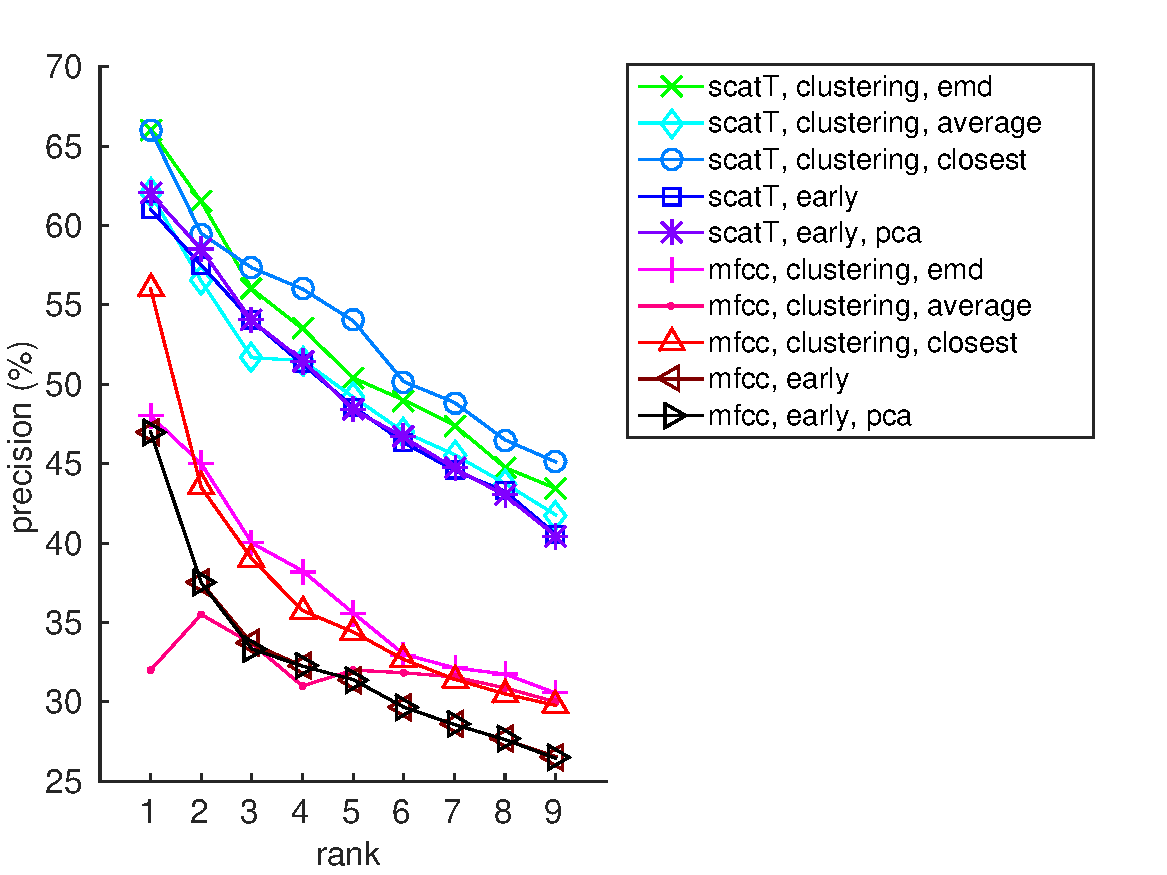
\includegraphics[width=\columnwidth]{figures/overall}
\caption{Acoustic scene similarity retrieval in the DCASE 2013 private dataset: precisions at rank $k$ ($p@k$) obtained for MFCCs and scattering with logarithmic compression.}
\label{fig:ASS_1}
\end{center}
\end{figure}

\subsubsection*{Sensitivity to number of clusters $M$}

We now study the sensitivity of the precision at rank $5$ ($p@5$) with respect to the number of clusters $M$.
The results are shown in Figure \ref{fig:sensitivityM}.

For a small number of clusters ($M = 1$ or $M = 2$), all methods perform worse, since not enough discriminative sound objects are extracted from the recording. Please note that setting $M = 1$ is equivalent to the \emph{early} approach as this corresponds a summary statistics model.
For $M = 4$, most methods perform well, since this allows for better characterization of various signal structures in the scenes.
As the number of clusters increases, the \emph{RbQ-a} method performs worse for both scattering features and MFCCs since any distinct objects are averaged out by clusters representing the background.
The \emph{RbQ-w} and \emph{RbQ-c} methods do better in this regard, as they are better able to emphasize the clusters that discriminate well between scenes.

Using \emph{RbQ-c}, therefore, we are not very sensitive to the choice of $M$, as long as it is large enough to allow for separation of the discriminative sound objects from the background.
This motivates our choice of $M = 8$ for the previous experiments in this section.

\begin{figure}[t]
\begin{center}
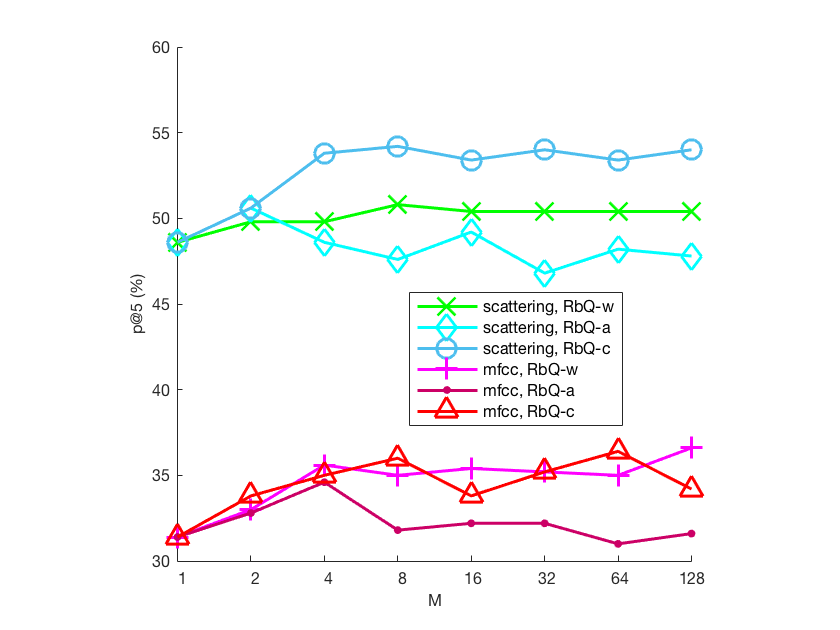
\includegraphics[width=\columnwidth]{figures/sensitivityM}
\caption{Acoustic scene similarity retrieval in the DCASE 2013 private dataset: precision at rank $5$ ($p@5$) obtained for different methods as a function of the number of clusters $M$.}
\label{fig:sensitivityM}
\end{center}
\end{figure}

\section{Conclusion}

This paper presents a new approach for modeling acoustic scenes based on scattering transforms at small scales and cluster-based representations at large scales. Compared to traditional BoF and summary statistics models, this representation allows for the characterization of distinct sound events superimposed on a stationary texture, a concept which has strong grounding in the cognitive psychology literature. To adequately capture such distinct events, we develop a cluster-based model and validate it using experiments on acoustic scene similarity retrieval. For this task, we show significant improvements over the traditional BoF and summary statistics models based on both standard MFCCs and scattering features.
These outcomes shall be studied further in future work by considering larger databases and emerging tasks in ecoacoustics~\cite{sueur2015ecoacoustics, wimmer2013sampling}.


\section*{Availability of data and materials}
The dataset supporting the conclusions of this article is available in the dcase2013 repository,  \sloppy \url{http://c4dm.eecs.qmul.ac.uk/sceneseventschallenge/description.html}.
The software supporting the conclusions of this article is available in
\begin{itemize}
\item \sloppy Companion website: \url{https://github.com/mathieulagrange/paperRelevanceBasedSimilarity}
\item Programming language: Matlab
\item License: GNU GPL
\item Any restrictions to use by non-academics: license needed
\end{itemize}


\section*{Competing interests}
The authors declare that they have no competing interests.

\section*{Funding}
This study is co-funded by the ANR under project reference ANR-16-CE22-0012.

\section*{Authors' contributions}
GL and VL carried out the numerical experiments and drafted the manuscript. VL, GL, JA and ML participated in the design of the study and helped to draft the manuscript.
All authors read and approved the final manuscript.


%\bibliographystyle{spmpsci}
%\bibliography{biblio}
\printbibliography


% \begin{IEEEbiography}[{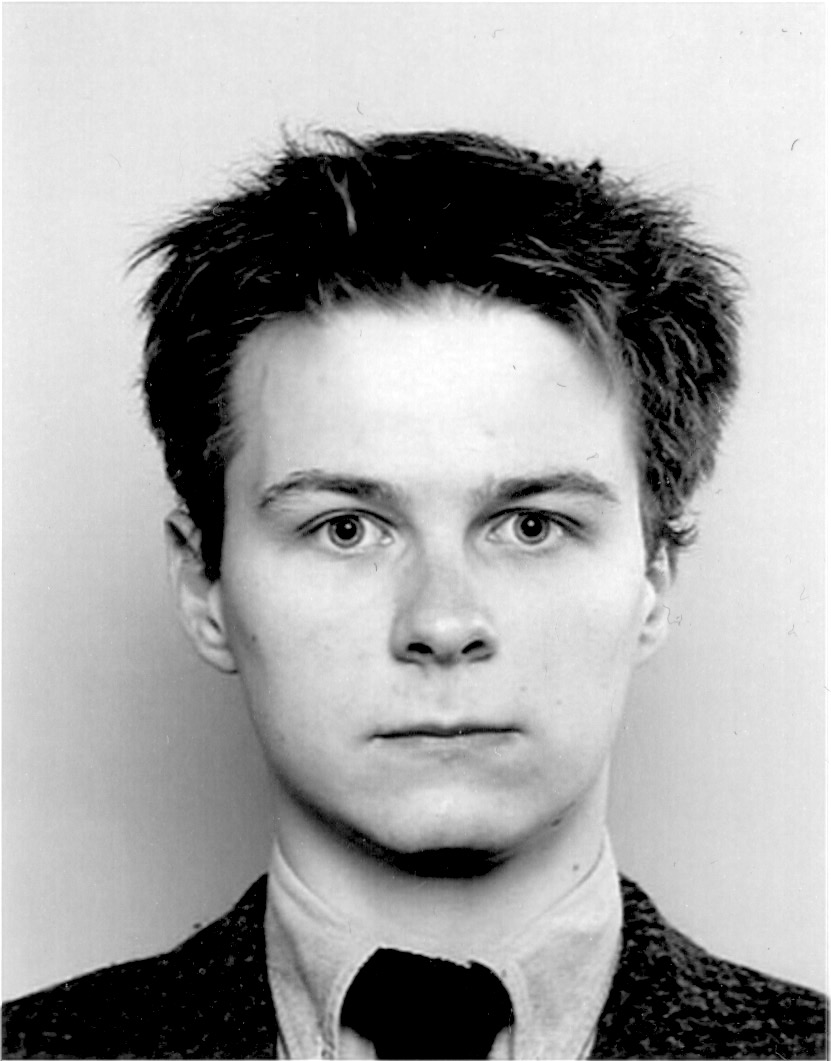
\includegraphics[width=1in,height=1.25in,clip,keepaspectratio]{figures/lostanlen}}]{Vincent Lostanlen} was born in 1992. He received an engineering degree from TELECOM ParisTech in 2013 and his M.S. degree in acoustics, signal processing, and musical informatics (ATIAM) from the Universit\'{e} Pierre et Marie Curie (UPMC) and the Ircam in Paris, France, in 2013. Since 2013, he is a Ph.D. student at \'{E}cole normale sup\'{e}rieure in Paris, working under the supervision of St\'{e}phane Mallat. His research focuses on defining convolutional operators in the time-frequency domain with applications in audio classification.
% \end{IEEEbiography}
%
% \begin{IEEEbiography}[{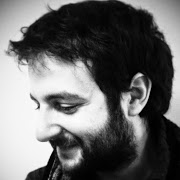
\includegraphics[width=1in,height=1.25in,clip,keepaspectratio]{figures/lafay}}]{Gr\'egoire Lafay} was born in 1990. He received the B.S. degree in Acoustic from the University Pierre and Marie Curie (UPMC), Paris, FranArthritis National Research Foundatioce, and the B.S. degree in Musicology from the Sorbonne University, Paris, France, in 2011. He received his M.S. degree in acoustics, signal processing, and musical informatics (ATIAM) from the UPMC and the Ircam in Paris, France, in 2013. Since 2013, he is a Ph.D. student at IRCCyN, Nantes, France. His research interests include acoustic scene similarity and classification as well as acoustic scene perception.
% \end{IEEEbiography}
%
%
% \begin{IEEEbiography}[{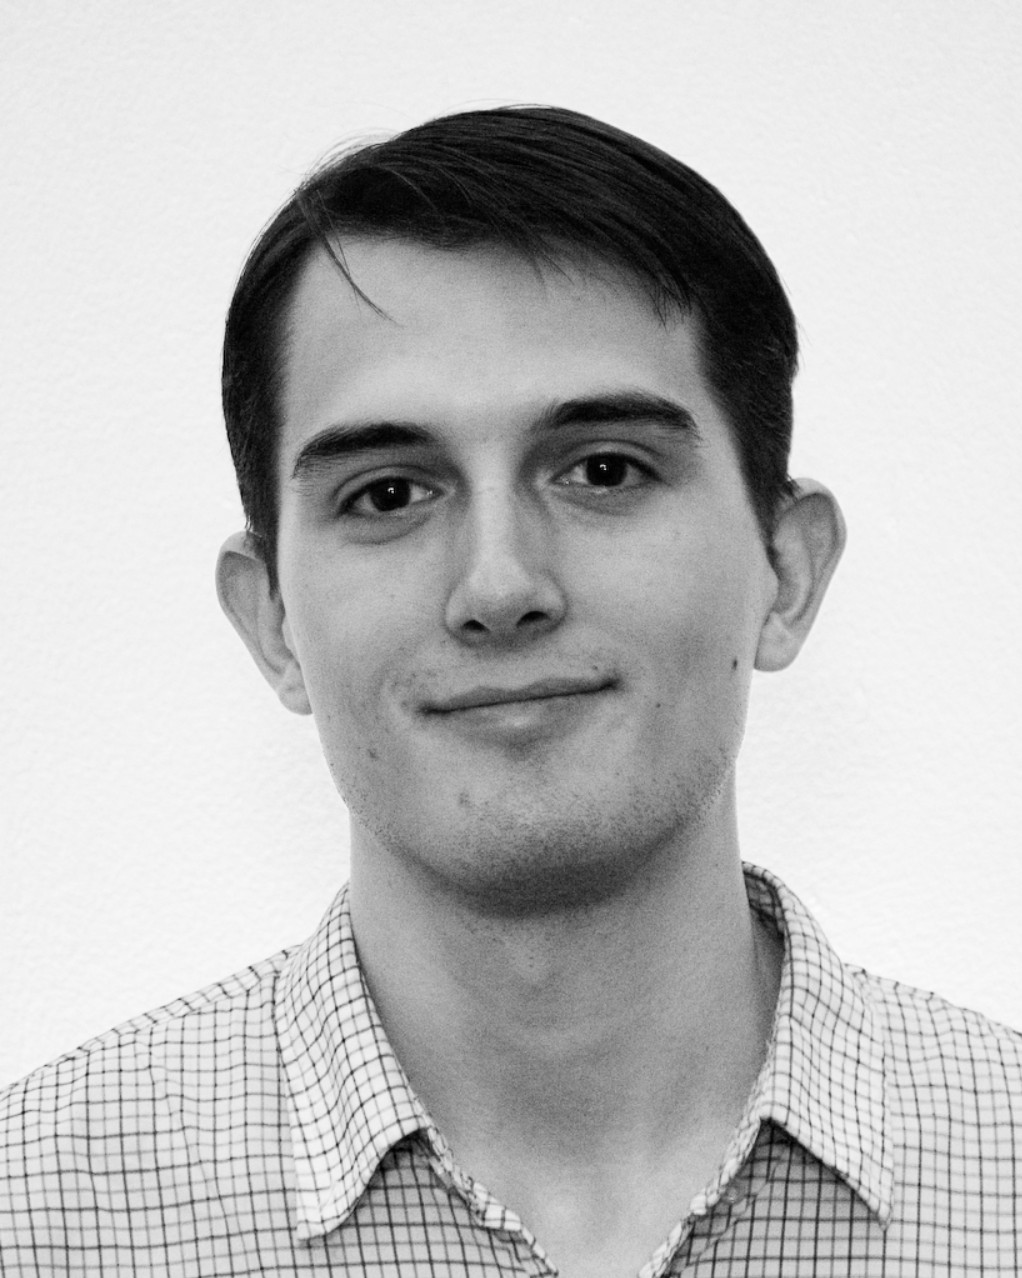
\includegraphics[width=1in,height=1.25in,clip,keepaspectratio]{figures/anden}}]{Joakim And\'en}
% received the M.Sc. degree in mathematics from the Universit\'e Pierre et Marie Curie, Paris, France, in 2010 and the Ph.D. degree in applied mathematics from Ecole Polytechnique, Palaiseau, France, in 2014. He is currently a postdoctoral researcher with the Program in Applied and Computational mathematics at Princeton University, Princeton, USA. His research interests include signal processing, machine learning, and statistical data analysis. He is a member of the IEEE.
%
% \end{IEEEbiography}
%
% \begin{IEEEbiography}[{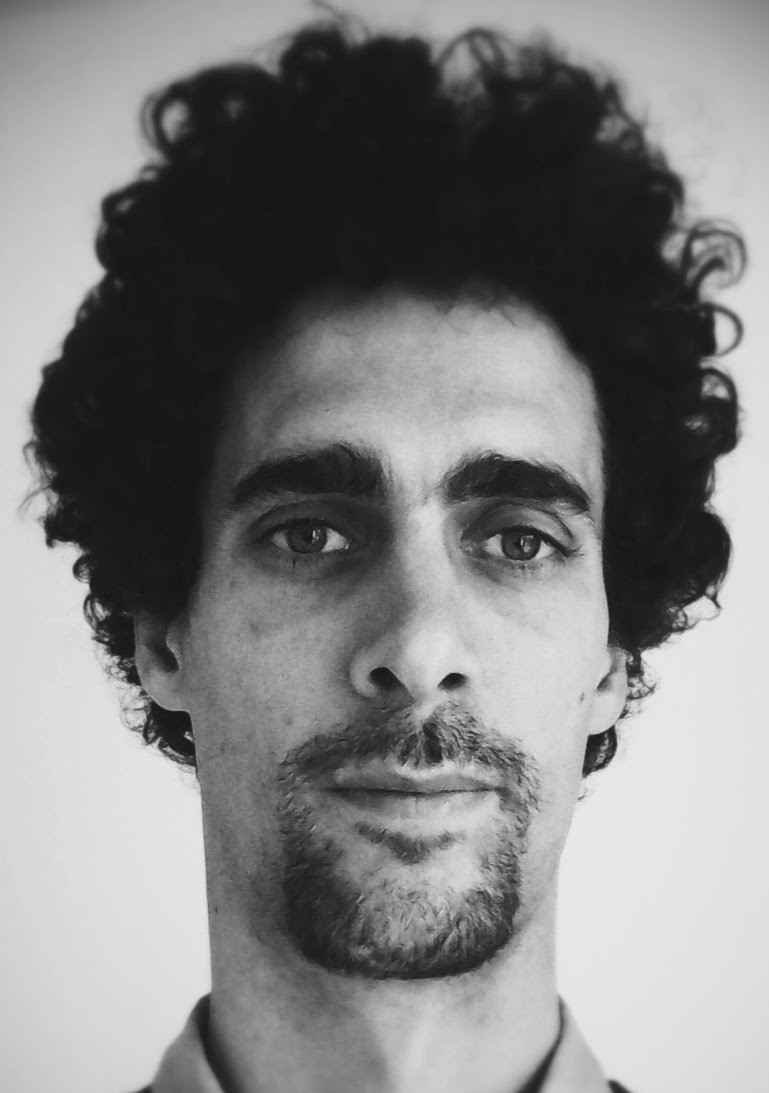
\includegraphics[width=1.25in,height=1.25in,clip,keepaspectratio]{figures/lagrange}}]{Mathieu Lagrange} is a CNRS research scientist at IRCCyN, a French laboratory dedicated to cybernetics. He obtained his Ph.D. in computer science at the University of Bordeaux in 2004, and visited several institutions in Canada (University of Victoria, McGill University) and in France (Orange Labs, TELECOM ParisTech, Ircam). His research focuses on machine listening algorithms applied to the analysis of musical and environmental audio.
% \end{IEEEbiography}

% biography section
%
% If you have an EPS/PDF photo (graphicx package needed) extra braces are
% needed around the contents of the optional argument to biography to prevent
% the LaTeX parser from getting confused when it sees the complicated
% \includegraphics command within an optional argument. (You could create
% your own custom macro containing the \includegraphics command to make things
% simpler here.)
%\begin{IEEEbiography}[{\includegraphics[width=1in,height=1.25in,clip,keepaspectratio]{mshell}}]{Michael Shell}
% or if you just want to reserve a space for a photo:

%\begin{IEEEbiography}{Mathieu Lagrange}
%Biography text here.
%\end{IEEEbiography}

% if you will not have a photo at all:
%\begin{IEEEbiographynophoto}{John Doe}
%Biography text here.
%\end{IEEEbiographynophoto}

% insert where needed to balance the two columns on the last page with
% biographies
%\newpage

%\begin{IEEEbiographynophoto}{Jane Doe}
%Biography text here.
%\end{IEEEbiographynophoto}

% You can push biographies down or up by placing
% a \vfill before or after them. The appropriate
% use of \vfill depends on what kind of text is
% on the last page and whether or not the columns
% are being equalized.

%\vfill

% Can be used to pull up biographies so that the bottom of the last one
% is flush with the other column.
%\enlargethispage{-5in}


\section{Supplementary material}

The asymmetric amplitude profile of Gammatones makes them suitable to model temporal masking in auditory filterbanks~\cite{Fastl2007}.
Yet, the introductory paper on Gammatone wavelets \cite{Venkitaraman2014} does not provide a formula for deducing $\sigma$ from the specification of a quality factor $Q$.
In this appendix, we provide a rationale for choosing the topmost center frequency $\xi$ of a Gammatone wavelet filter bank in a discrete-time setting. Then, we relate the bandwidth parameter $\sigma$ to the choice of a quality factor Q.


\subsubsection*{Motivation}
Time reversal of a real signal $\boldsymbol{x}(t)$ is equivalent
to the complex conjugation of its Fourier transform $\boldsymbol{\widehat{x}}(\omega$).
As a consequence, the Fourier transform modulus $\vert\boldsymbol{\widehat{x}}(\omega)\vert$
is not only invariant to translation, but also invariant to time reversal.
Yet, although invariance to translation is needed for classification,
invariance to time reversal is an undesirable property.
A simple way to break invariance to time reversal is to choose $\boldsymbol{\psi}(t)$
as an asymmetric wavelet instead of a Gabor symmetric wavelet.

The complex-valued Gammatone wavelet is a modification of the real-valued
Gammatone auditory filter, originated in auditory physiology. The
Gammatone auditory filter of dimensionless frequency $1$ is defined
as a gamma distribution of order $N\in\mathbb{N}^{*}$ and bandwidth
$\sigma$ modulated by a sine wave, that is,
\[
t^{N-1}\exp(-2\pi\sigma t)\cos(2\pi t).
\]
For a fixed $\sigma$, the integer $N$ controls the relative shape
of the envelope, becoming less skewed as $N$ increases. Psychoacoustical
experiments have shown that, for $N=4$, the Gammatone function provides
a valid approximation of the basilar membrane response in the mammalian
cochlea \cite{Flanagan1960,Patterson1976,Lyon2010}. In particular,
it is asymmetric both in the time domain and in the Fourier domain,
which allows to reproduce the asymmetry of temporal masking as well
as the asymmetry of spectral masking \cite{Fastl2007}. It is thus
used in computational models for auditory physiology \cite{Pressnitzer2005}.
However, it does not comply with the Grossman-Morlet admissibility
condition, because it has a non-negligible average. In addition, because
the Gammatone auditory filter takes real values in the time domain,
its Fourier transform satisfies Hermitian symmetry, which implies
that it does not belong to the space $H^{2}$ of analytic functions.
More generally, there are no real-valued functions in $H^{2}$ \cite{Grossmann1984}.

\subsubsection*{Related work}

With the aim of building a pseudo-analytic admissible Gammatone wavelet,
\cite{Venkitaraman2014} have modified the definition of the Gammatone
auditory filter, by replacing the real-valued sine wave $\cos(2\pi t)$
by its analytic part $\exp(2\pi\mathrm{\mathrm{i}}t)$ and by taking
the first derivative of the gamma distribution, thus ensuring null
mean. The definition of the Gammatone wavelet becomes
\[
\boldsymbol{\psi}(t)=\left(2\pi(\mathrm{i}-\sigma)t^{N-1}+(N-1)t^{N-2}\right)\exp(-2\pi\sigma t)\exp(2\pi\mathrm{i}t)
\]
in the time domain, and
\[
\boldsymbol{\widehat{\psi}}(\omega)=\dfrac{\mathrm{i}\omega\times(N-1)!}{(\sigma+\mathrm{i}(\omega-\sigma))^{N}}
\]
in the Fourier domain. Besides its biological plausibility, the Gammatone
wavelet enjoys a near-optimal time-frequency localization with respect
to the Heisenberg uncertainty principle. Furthermore, this time-frequency
localization tends to optimality as $N$ approaches infinity, because
the limit $N\rightarrow+\infty$ yields a Gabor wavelet \cite{Cohen1995}.
Last but not least, the Gammatone wavelet transform of finite order
$N$ is causal, as opposed to the Morlet wavelet transform, which
makes it better suited to real-time applications. From an evolutionary
point of view, it has been argued that the Gammatone reaches a practical
compromise between time-frequency localization and causality constraints \cite{Venkitaraman2014}.


\subsubsection*{Center frequency parameter}

In order to preserve energy and allow for perfect reconstruction,
the Gammatone wavelet filter bank must satisfy the inequalities
\[
1-\varepsilon\leq\vert\boldsymbol{\hat{\phi}}(\omega)\vert+\sum_{\gamma}\vert\boldsymbol{\hat{\psi}}(2^{\gamma}\omega)\vert+\vert\boldsymbol{\hat{\psi}}(-2^{\gamma}\omega)\vert\leq1
\]
for all frequencies $\omega$, where $\varepsilon$ is a small margin
\cite{Anden2014}. Satisfying the equation above near the Nyquist
frequency $\omega=\pi$ can be achieved by placing the log-frequency
$\log_{2}\xi$ of the first (topmost) wavelet in between the log-frequency
$\log_{2}(\xi\times2^{-1/Q})$ of the second wavelet and the log-frequency
$\log_{2}(2\pi-\xi)$ of the mirror of the first wavelet. We obtain
the equation
\[
\log_{2}\xi-\log_{2}(\xi\times2^{-1/Q})=\log_{2}(2\pi-\xi)-\log_{2}\xi,
\]

of which we deduce the identity
\[
\xi=\dfrac{2\pi}{1+2^{1/Q}}.
\]
For $Q=1$, this yields a center frequency of $\xi=\frac{2\pi}{3}$.
For greater values of $Q$, the center frequency $\xi$ tends towards
$\pi$.


\subsubsection*{Bandwidth parameter}

The quality factor $Q$ of the Gammatone wavelet is defined as the
ratio between the center frequency $\xi$ of the wavelet $\boldsymbol{\hat{\psi}}(\omega)$
and its bandwidth $B$ in the Fourier domain. This bandwidth is given
by the difference between the two solutions $\omega$ of the following
equation:

\[
\dfrac{\vert\boldsymbol{\hat{\psi}}(\omega)\vert}{\vert\boldsymbol{\hat{\psi}}(\xi)\vert}=\dfrac{\omega}{\xi}\times\left(1+\dfrac{\left(\omega-\xi\right)^{2}}{\sigma^{2}}\right)^{-N/2}=r,
\]
where the magnitude cutoff $r$ is most
often set to $\sqrt{\frac{1}{2}}$. Let $\Delta\omega=\omega-\xi$.
Raising the above equation to the power $N/2$ yields the following:
\[
\left(1+\dfrac{\Delta\omega}{\omega_{c}}\right)^{N/2}=r\times\left(1+\frac{\Delta\omega^{2}}{\alpha^{2}}\right).
\]
Since $\Delta\omega\ll\xi$, we may approximate the left-hand side
with a first-order Taylor expansion. This leads to a quadratic equation
of the variable $\Delta\negmedspace\omega$:
\[
\dfrac{r^{2/N}}{\sigma^{2}}\times\Delta\omega^{2}-\dfrac{2}{N\xi}\times\Delta\omega+\left(r^{2/N}-1\right)=0.
\]
The discriminant of the above equation is:
\[
D=4\times\left(\dfrac{1}{N^{2}\xi^{2}}+\dfrac{r^{2/N}\left(1-r^{2/N}\right)}{\sigma^{2}}\right),
\]
which is a positive number as long as $r<1$. The bandwidth $B$ of
$\boldsymbol{\hat{\psi}}$ is given by the difference between the
two solutions of the quadratic equation, that is:
\[
B=\dfrac{2\sigma^{2}}{r^{2/N}}\times\sqrt{\dfrac{1}{N^{2}\xi^{2}}+\dfrac{r^{2/N}\left(1-r^{2/N}\right)}{\sigma^{2}}}.
\]
Now, let us express the parameter $\alpha$ as a function of some
required bandwidth $B$ at some cutoff threshold $r$. After having
raised the above to its square and rearranged the terms, we obtain
another quadratic equation, yet of the variable $\mbox{\ensuremath{\alpha}}^{2}$:
\[
\dfrac{4}{r^{4/N}N^{2}\xi^{2}}\sigma^{4}+\dfrac{4\times\left(1-r^{2/N}\right)}{r^{2/N}}\sigma^{2}-B^{2}=0
\]
We multiply the equation by $\dfrac{r^{2/N}}{4\times\left(1-r^{2/N}\right)}\neq0:$
\[
\dfrac{1}{r^{2/N}\left(1-r^{2/N}\right)N^{2}\xi^{2}}\sigma^{4}+\sigma^{2}-\dfrac{r^{2/N}B^{2}}{4\times\left(1-r^{2/N}\right)}=0
\]
This leads to defining $\sigma^{2}$ as the unique positive root of
the above polynomial:
\[
\sigma^{2}=\dfrac{r^{2/N}\left(1-r^{2/N}\right)N^{2}\xi^{2}}{2}\times\left(\sqrt{1+\dfrac{B^{2}}{\left(1-r^{2/N}\right)^{2}N^{2}\xi^{2}}}-1\right).
\]
If the filter bank has to be approximately orthogonal, we typically
set $B$ to $B=\left(1-2^{-1/Q}\right)\times\xi$.

We conclude with the following closed form for $\alpha$:
\[
\alpha=K_{N}\times\sqrt{\dfrac{\sqrt{1+h_{N}\left(Q\right)^{2}}-1}{2}}\times\xi,
\]
where
\[
K_{N}=r^{1/N}N\sqrt{1-r^{2/N}}\mbox{ and }h_{N}\left(Q\right)=\dfrac{1-2^{-1/Q}}{N\times\left(1-r^{2/N}\right)}.
\]





% that's all folks
\end{document}
